\documentclass{ximera}

%\usepackage{todonotes}

\newcommand{\todo}{}

\usepackage{esint} % for \oiint
\ifxake%%https://math.meta.stackexchange.com/questions/9973/how-do-you-render-a-closed-surface-double-integral
\renewcommand{\oiint}{{\large\bigcirc}\kern-1.56em\iint}
\fi


\graphicspath{
  {./}
  {ximeraTutorial/}
  {basicPhilosophy/}
  {functionsOfSeveralVariables/}
  {normalVectors/}
  {lagrangeMultipliers/}
  {vectorFields/}
  {greensTheorem/}
  {shapeOfThingsToCome/}
  {dotProducts/}
  {partialDerivativesAndTheGradientVector/}
  {../productAndQuotientRules/exercises/}
  {../normalVectors/exercisesParametricPlots/}
  {../continuityOfFunctionsOfSeveralVariables/exercises/}
  {../partialDerivativesAndTheGradientVector/exercises/}
  {../directionalDerivativeAndChainRule/exercises/}
  {../commonCoordinates/exercisesCylindricalCoordinates/}
  {../commonCoordinates/exercisesSphericalCoordinates/}
  {../greensTheorem/exercisesCurlAndLineIntegrals/}
  {../greensTheorem/exercisesDivergenceAndLineIntegrals/}
  {../shapeOfThingsToCome/exercisesDivergenceTheorem/}
  {../greensTheorem/}
  {../shapeOfThingsToCome/}
  {../separableDifferentialEquations/exercises/}
  {vectorFields/}
}

\newcommand{\mooculus}{\textsf{\textbf{MOOC}\textnormal{\textsf{ULUS}}}}

\usepackage{tkz-euclide}
\usepackage{tikz}
\usepackage{tikz-cd}
\usetikzlibrary{arrows}
\tikzset{>=stealth,commutative diagrams/.cd,
  arrow style=tikz,diagrams={>=stealth}} %% cool arrow head
\tikzset{shorten <>/.style={ shorten >=#1, shorten <=#1 } } %% allows shorter vectors

\usetikzlibrary{backgrounds} %% for boxes around graphs
\usetikzlibrary{shapes,positioning}  %% Clouds and stars
\usetikzlibrary{matrix} %% for matrix
\usepgfplotslibrary{polar} %% for polar plots
\usepgfplotslibrary{fillbetween} %% to shade area between curves in TikZ
%\usetkzobj{all}
\usepackage[makeroom]{cancel} %% for strike outs
%\usepackage{mathtools} %% for pretty underbrace % Breaks Ximera
%\usepackage{multicol}
\usepackage{pgffor} %% required for integral for loops



%% http://tex.stackexchange.com/questions/66490/drawing-a-tikz-arc-specifying-the-center
%% Draws beach ball
\tikzset{pics/carc/.style args={#1:#2:#3}{code={\draw[pic actions] (#1:#3) arc(#1:#2:#3);}}}



\usepackage{array}
\setlength{\extrarowheight}{+.1cm}
\newdimen\digitwidth
\settowidth\digitwidth{9}
\def\divrule#1#2{
\noalign{\moveright#1\digitwidth
\vbox{\hrule width#2\digitwidth}}}




% \newcommand{\RR}{\mathbb R}
% \newcommand{\R}{\mathbb R}
% \newcommand{\N}{\mathbb N}
% \newcommand{\Z}{\mathbb Z}

\newcommand{\sagemath}{\textsf{SageMath}}


%\renewcommand{\d}{\,d\!}
%\renewcommand{\d}{\mathop{}\!d}
%\newcommand{\dd}[2][]{\frac{\d #1}{\d #2}}
%\newcommand{\pp}[2][]{\frac{\partial #1}{\partial #2}}
% \renewcommand{\l}{\ell}
%\newcommand{\ddx}{\frac{d}{\d x}}

% \newcommand{\zeroOverZero}{\ensuremath{\boldsymbol{\tfrac{0}{0}}}}
%\newcommand{\inftyOverInfty}{\ensuremath{\boldsymbol{\tfrac{\infty}{\infty}}}}
%\newcommand{\zeroOverInfty}{\ensuremath{\boldsymbol{\tfrac{0}{\infty}}}}
%\newcommand{\zeroTimesInfty}{\ensuremath{\small\boldsymbol{0\cdot \infty}}}
%\newcommand{\inftyMinusInfty}{\ensuremath{\small\boldsymbol{\infty - \infty}}}
%\newcommand{\oneToInfty}{\ensuremath{\boldsymbol{1^\infty}}}
%\newcommand{\zeroToZero}{\ensuremath{\boldsymbol{0^0}}}
%\newcommand{\inftyToZero}{\ensuremath{\boldsymbol{\infty^0}}}



% \newcommand{\numOverZero}{\ensuremath{\boldsymbol{\tfrac{\#}{0}}}}
% \newcommand{\dfn}{\textbf}
% \newcommand{\unit}{\,\mathrm}
% \newcommand{\unit}{\mathop{}\!\mathrm}
% \newcommand{\eval}[1]{\bigg[ #1 \bigg]}
% \newcommand{\seq}[1]{\left( #1 \right)}
% \renewcommand{\epsilon}{\varepsilon}
% \renewcommand{\phi}{\varphi}


% \renewcommand{\iff}{\Leftrightarrow}

% \DeclareMathOperator{\arccot}{arccot}
% \DeclareMathOperator{\arcsec}{arcsec}
% \DeclareMathOperator{\arccsc}{arccsc}
% \DeclareMathOperator{\si}{Si}
% \DeclareMathOperator{\scal}{scal}
% \DeclareMathOperator{\sign}{sign}


%% \newcommand{\tightoverset}[2]{% for arrow vec
%%   \mathop{#2}\limits^{\vbox to -.5ex{\kern-0.75ex\hbox{$#1$}\vss}}}
% \newcommand{\arrowvec}[1]{{\overset{\rightharpoonup}{#1}}}
% \renewcommand{\vec}[1]{\arrowvec{\mathbf{#1}}}
% \renewcommand{\vec}[1]{{\overset{\boldsymbol{\rightharpoonup}}{\mathbf{#1}}}}

% \newcommand{\point}[1]{\left(#1\right)} %this allows \vector{ to be changed to \vector{ with a quick find and replace
% \newcommand{\pt}[1]{\mathbf{#1}} %this allows \vec{ to be changed to \vec{ with a quick find and replace
% \newcommand{\Lim}[2]{\lim_{\point{#1} \to \point{#2}}} %Bart, I changed this to point since I want to use it.  It runs through both of the exercise and exerciseE files in limits section, which is why it was in each document to start with.

% \DeclareMathOperator{\proj}{\mathbf{proj}}
% \newcommand{\veci}{{\boldsymbol{\hat{\imath}}}}
% \newcommand{\vecj}{{\boldsymbol{\hat{\jmath}}}}
% \newcommand{\veck}{{\boldsymbol{\hat{k}}}}
% \newcommand{\vecl}{\vec{\boldsymbol{\l}}}
% \newcommand{\uvec}[1]{\mathbf{\hat{#1}}}
% \newcommand{\utan}{\mathbf{\hat{t}}}
% \newcommand{\unormal}{\mathbf{\hat{n}}}
% \newcommand{\ubinormal}{\mathbf{\hat{b}}}

% \newcommand{\dotp}{\bullet}
% \newcommand{\cross}{\boldsymbol\times}
% \newcommand{\grad}{\boldsymbol\nabla}
% \newcommand{\divergence}{\grad\dotp}
% \newcommand{\curl}{\grad\cross}
%\DeclareMathOperator{\divergence}{divergence}
%\DeclareMathOperator{\curl}[1]{\grad\cross #1}
% \newcommand{\lto}{\mathop{\longrightarrow\,}\limits}

% \renewcommand{\bar}{\overline}

\colorlet{textColor}{black}
\colorlet{background}{white}
\colorlet{penColor}{blue!50!black} % Color of a curve in a plot
\colorlet{penColor2}{red!50!black}% Color of a curve in a plot
\colorlet{penColor3}{red!50!blue} % Color of a curve in a plot
\colorlet{penColor4}{green!50!black} % Color of a curve in a plot
\colorlet{penColor5}{orange!80!black} % Color of a curve in a plot
\colorlet{penColor6}{yellow!70!black} % Color of a curve in a plot
\colorlet{fill1}{penColor!20} % Color of fill in a plot
\colorlet{fill2}{penColor2!20} % Color of fill in a plot
\colorlet{fillp}{fill1} % Color of positive area
\colorlet{filln}{penColor2!20} % Color of negative area
\colorlet{fill3}{penColor3!20} % Fill
\colorlet{fill4}{penColor4!20} % Fill
\colorlet{fill5}{penColor5!20} % Fill
\colorlet{gridColor}{gray!50} % Color of grid in a plot

\newcommand{\surfaceColor}{violet}
\newcommand{\surfaceColorTwo}{redyellow}
\newcommand{\sliceColor}{greenyellow}




\pgfmathdeclarefunction{gauss}{2}{% gives gaussian
  \pgfmathparse{1/(#2*sqrt(2*pi))*exp(-((x-#1)^2)/(2*#2^2))}%
}


%%%%%%%%%%%%%
%% Vectors
%%%%%%%%%%%%%

%% Simple horiz vectors
\renewcommand{\vector}[1]{\left\langle #1\right\rangle}


%% %% Complex Horiz Vectors with angle brackets
%% \makeatletter
%% \renewcommand{\vector}[2][ , ]{\left\langle%
%%   \def\nextitem{\def\nextitem{#1}}%
%%   \@for \el:=#2\do{\nextitem\el}\right\rangle%
%% }
%% \makeatother

%% %% Vertical Vectors
%% \def\vector#1{\begin{bmatrix}\vecListA#1,,\end{bmatrix}}
%% \def\vecListA#1,{\if,#1,\else #1\cr \expandafter \vecListA \fi}

%%%%%%%%%%%%%
%% End of vectors
%%%%%%%%%%%%%

%\newcommand{\fullwidth}{}
%\newcommand{\normalwidth}{}



%% makes a snazzy t-chart for evaluating functions
%\newenvironment{tchart}{\rowcolors{2}{}{background!90!textColor}\array}{\endarray}

%%This is to help with formatting on future title pages.
\newenvironment{sectionOutcomes}{}{}



%% Flowchart stuff
%\tikzstyle{startstop} = [rectangle, rounded corners, minimum width=3cm, minimum height=1cm,text centered, draw=black]
%\tikzstyle{question} = [rectangle, minimum width=3cm, minimum height=1cm, text centered, draw=black]
%\tikzstyle{decision} = [trapezium, trapezium left angle=70, trapezium right angle=110, minimum width=3cm, minimum height=1cm, text centered, draw=black]
%\tikzstyle{question} = [rectangle, rounded corners, minimum width=3cm, minimum height=1cm,text centered, draw=black]
%\tikzstyle{process} = [rectangle, minimum width=3cm, minimum height=1cm, text centered, draw=black]
%\tikzstyle{decision} = [trapezium, trapezium left angle=70, trapezium right angle=110, minimum width=3cm, minimum height=1cm, text centered, draw=black]


\title{Behavior}

\begin{document}

\begin{abstract}
increasing and decreasing
\end{abstract}
\maketitle



Probably the most important characteristic we want to know about a function is its behaviore.  That is, where is it increasing and where is it decreasing? \\




Increasing and decreasing for a function is a comparison between its domain and range, which are both a set of numbers.  So, to understand function behavior, we need to first understand number behavior.



\textbf{\textcolor{blue!55!black}{Number Behavior:}}  Our real numbers have a natural ordering, which we call \textit{less than} and \textit{greater than}.  Visually, these mean ``to the left of'' and ``to the right of'' on a number line. \\

If you move to the right on the number line, then the numbers are increasing. \\

If you move to the left on the number line, then the numbers are decreasing. \\











With functions, we have two number lines and we compare movement on them to each other. \\










\begin{template} \textbf{\textcolor{blue!55!black}{Increasing Function}} 


A function is increasing if its domain and range values change in the same way. \\


In other words, when we move to the right on the domain number line, the corresponding movement on the range number line is also to the right.

When the domain increases, the function values also increase.


Graphically, we have to remember that our range number line is not horizontal.  It is vertical.  When we move to the right on the domain number line, then the corresponding movement on the range number line is up.



\[
\text{ When } \,  a < b \, \text{ then } \, f(a) < f(b)
\]


\end{template}














\begin{template} \textbf{\textcolor{blue!55!black}{Decreasing Function}} 


A function is decreasing if its domain and range values change in oppositely. \\


In other words, when we move to the right on the domain number line, the corresponding movement on the range number line is to the left.

When the domain increases, the function values decrease.


Graphically, we have to remember that our range number line is not horizontal.  It is vertical.  When we move to the right on the domain number line, then the corresponding movement on the range number line is down.



\[
\text{ When } \,  a < b \, \text{ then } \, f(a) > f(b)
\]


\end{template}






We want to following this idea through compositions.   \\






\subsection*{Increasing $\circ$ Increasing}



$f$ and $g$ are defined graphically below.  They are both increasing functions. \\

What about $f \circ g$? \\



\begin{image}
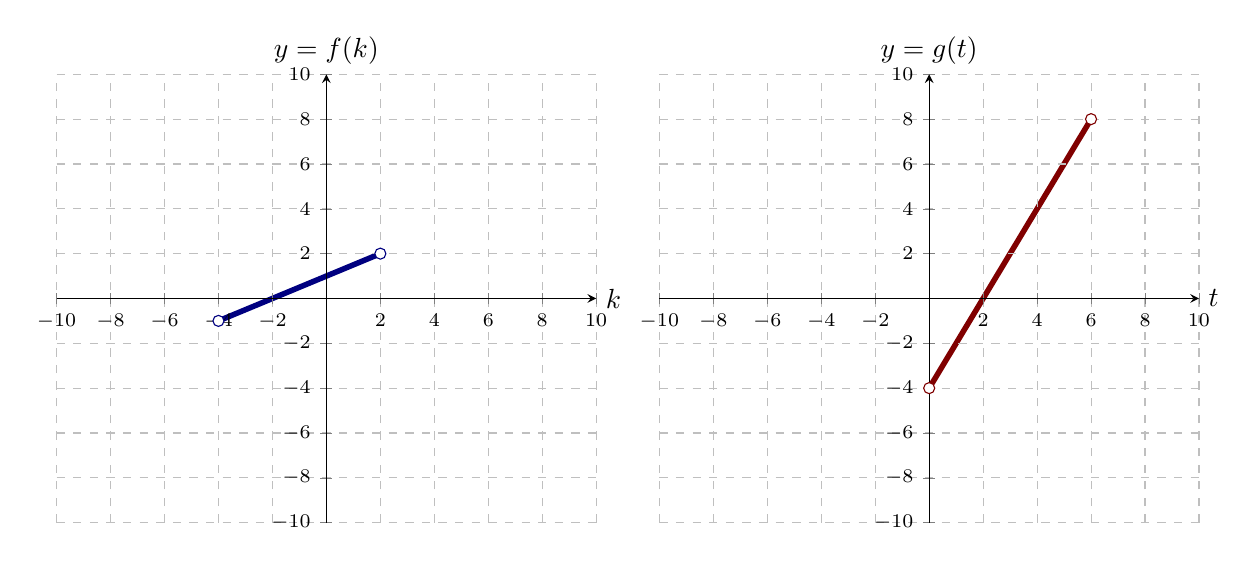
\begin{tikzpicture}
    \begin{axis}[name = sinax, domain=-10:10, ymax=10, xmax=10, ymin=-10, xmin=-10,
            axis lines =center, xlabel=$k$, ylabel={$y=f(k)$}, grid = major, grid style={dashed},
            ytick={-10,-8,-6,-4,-2,2,4,6,8,10},
            xtick={-10,-8,-6,-4,-2,2,4,6,8,10},
            yticklabels={$-10$,$-8$,$-6$,$-4$,$-2$,$2$,$4$,$6$,$8$,$10$}, 
            xticklabels={$-10$,$-8$,$-6$,$-4$,$-2$,$2$,$4$,$6$,$8$,$10$},
            ticklabel style={font=\scriptsize},
            every axis y label/.style={at=(current axis.above origin),anchor=south},
            every axis x label/.style={at=(current axis.right of origin),anchor=west},
            axis on top
          ]
          
          \addplot [line width=2, penColor, smooth,samples=100,domain=(-4:2)] ({x},{0.5*x+1});
          \addplot [color=penColor,fill=background, only marks,mark=*] coordinates{(-4,-1)};
          \addplot [color=penColor,fill=background, only marks,mark=*] coordinates{(2,2)}; 

           

    \end{axis}
    \begin{axis}[at={(sinax.outer east)},anchor=outer west, domain=-10:10, ymax=10, xmax=10, ymin=-10, xmin=-10,
            axis lines =center, xlabel=$t$, ylabel={$y=g(t)$}, grid = major, grid style={dashed},
            ytick={-10,-8,-6,-4,-2,2,4,6,8,10},
            xtick={-10,-8,-6,-4,-2,2,4,6,8,10},
            yticklabels={$-10$,$-8$,$-6$,$-4$,$-2$,$2$,$4$,$6$,$8$,$10$}, 
            xticklabels={$-10$,$-8$,$-6$,$-4$,$-2$,$2$,$4$,$6$,$8$,$10$},
            ticklabel style={font=\scriptsize},
            every axis y label/.style={at=(current axis.above origin),anchor=south},
            every axis x label/.style={at=(current axis.right of origin),anchor=west},
            axis on top
          ]
          
          \addplot [line width=2, penColor2, smooth,samples=100,domain=(0:6)] ({x},{2*x-4});
          \addplot [color=penColor2,fill=background, only marks,mark=*] coordinates{(0,-4)};
          \addplot [color=penColor2,fill=background, only marks,mark=*] coordinates{(6,8)}; 


  \end{axis}

\end{tikzpicture}
\end{image}



To decide the function behavior of a composition, we need to follow movement through two graphs. \\



\[
(f \circ g)(x) = f(g(x))
\]



\textbf{\textcolor{blue!55!black}{Domain Movement in $g$:}}  First, we think of movement to the right in the domain of $f \circ g$.  This would be movement to the right in the domain of $g$.  The graph of $g$ is on the right above.  This would be movement to the right on the horizontal axis.



\textbf{\textcolor{blue!55!black}{Range Movement in $g$:}}  Next, according to the graph of $g$, as we move the right in the domain of $g$, the values of $g$ move up, which is to the right in the range of $g$.




\textbf{\textcolor{blue!55!black}{switch:}}   The range of $g$ becomes the domain of $f$.  


\textbf{\textcolor{blue!55!black}{Domain Movement in $f$:}}   The range of $g$ becomes the domain of $f$.  We were moving up on the graph of $g$, which means to the right in the range of $g$.  This switches to movement to the right in the domain of $f$.


\textbf{\textcolor{blue!55!black}{Range Movement in $f$:}}  Next, according to the graph of $f$, as we move the right in the domain of $f$, the values of $f$ move up, which is to the right in the range of $f$.  This is the range of $f \circ g$.




Gluing the whole story, movement to the right in the domain of $f \circ g$ corresponds to movement to the right in the range of $f \circ g$.

$f \circ g$ is an increasing function.



\begin{observation}


This only applies to the domain of $f \circ g$, which needs to be determined. \\



The range of $g$ is $(-4, 8)$.  However, the domain of $f$ is $(-4, 2)$.   We cannot use the whole range of $g$, which means we cannot use the whole domain of $g$.  Which part of the domain of $g$ does $g$ map into $(-4, 2)$? \\


We need solutions to $g(t) = 2$.  From the graph, it looks like $g(3) = 2$.  Therefore, we can only use $(0, 3)$ from the domain of $g$.


Therefore, the domain of $f \circ g$ is $(0, 3)$.  On this domain, $f \circ g$ is increasing.



\end{observation}




\begin{warning}

Increasing means the domain and range change in the same way.

When the domain increases, then range increases.

It goes the other way as well.

When the domain decreases, the range decreases.

They mean the same thing.


\end{warning}



We can describe all of this thinking algebraically as well. \\


If $a < b$ in the domain of $f \circ g$, then we want to know about $(f \circ g)(a)$  and $(f \circ g)(b)$.



\textbf{Step 1:}  If $a < b$, then $g(a) < g(b)$, because $g$ is an increasing function.


\textbf{Step 2:}  Now think of $g(a)$  and $g(b)$ as domain numbers for $f$.


\textbf{Step 3:}  If $g(a) < g(b)$, then $f(g(a)) < f(g(b))$, because $f$ is an incresing function.


\textbf{Beginning to End:} If $a < b$, then $f(g(a)) < f(g(b))$ and $f \circ g$ is an increasing function.




















\subsection*{Increasing $\circ$ Decreasing}



$f$ and $g$ are defined graphically below.  $f$ is an increasing function.  $g$ is a decreasing function. \\

What about $f \circ g$? \\



\begin{image}
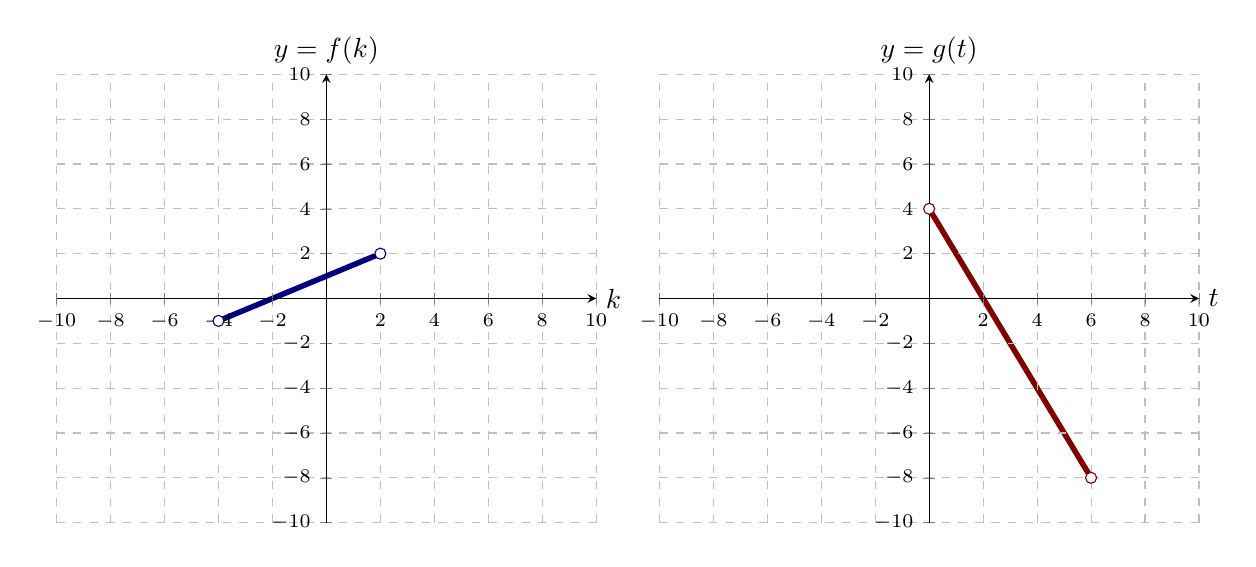
\begin{tikzpicture}
    \begin{axis}[name = sinax, domain=-10:10, ymax=10, xmax=10, ymin=-10, xmin=-10,
            axis lines =center, xlabel=$k$, ylabel={$y=f(k)$}, grid = major, grid style={dashed},
            ytick={-10,-8,-6,-4,-2,2,4,6,8,10},
            xtick={-10,-8,-6,-4,-2,2,4,6,8,10},
            yticklabels={$-10$,$-8$,$-6$,$-4$,$-2$,$2$,$4$,$6$,$8$,$10$}, 
            xticklabels={$-10$,$-8$,$-6$,$-4$,$-2$,$2$,$4$,$6$,$8$,$10$},
            ticklabel style={font=\scriptsize},
            every axis y label/.style={at=(current axis.above origin),anchor=south},
            every axis x label/.style={at=(current axis.right of origin),anchor=west},
            axis on top
          ]
          
          \addplot [line width=2, penColor, smooth,samples=100,domain=(-4:2)] ({x},{0.5*x+1});
          \addplot [color=penColor,fill=background, only marks,mark=*] coordinates{(-4,-1)};
          \addplot [color=penColor,fill=background, only marks,mark=*] coordinates{(2,2)}; 

           

    \end{axis}
    \begin{axis}[at={(sinax.outer east)},anchor=outer west, domain=-10:10, ymax=10, xmax=10, ymin=-10, xmin=-10,
            axis lines =center, xlabel=$t$, ylabel={$y=g(t)$}, grid = major, grid style={dashed},
            ytick={-10,-8,-6,-4,-2,2,4,6,8,10},
            xtick={-10,-8,-6,-4,-2,2,4,6,8,10},
            yticklabels={$-10$,$-8$,$-6$,$-4$,$-2$,$2$,$4$,$6$,$8$,$10$}, 
            xticklabels={$-10$,$-8$,$-6$,$-4$,$-2$,$2$,$4$,$6$,$8$,$10$},
            ticklabel style={font=\scriptsize},
            every axis y label/.style={at=(current axis.above origin),anchor=south},
            every axis x label/.style={at=(current axis.right of origin),anchor=west},
            axis on top
          ]
          
          \addplot [line width=2, penColor2, smooth,samples=100,domain=(0:6)] ({x},{-2*x+4});
          \addplot [color=penColor2,fill=background, only marks,mark=*] coordinates{(0,4)};
          \addplot [color=penColor2,fill=background, only marks,mark=*] coordinates{(6,-8)}; 


  \end{axis}

\end{tikzpicture}
\end{image}



To decide the function behavior of a composition, we need to follow movement through two graphs. \\



\[
(f \circ g)(x) = f(g(x))
\]



\textbf{\textcolor{blue!55!black}{Domain Movement in $g$:}}  First, we think of movement to the right in the domain of $f \circ g$.  This would be movement to the right in the domain of $g$.  The graph of $g$ is on the right above.  This would be movement to the right on the horizontal axis.



\textbf{\textcolor{blue!55!black}{Range Movement in $g$:}}  Next, according to the graph of $g$, as we move the right in the domain of $g$, the values of $g$ move down, which is to the left in the range of $g$.




\textbf{\textcolor{blue!55!black}{switch:}}   The range of $g$ becomes the domain of $f$.  


\textbf{\textcolor{blue!55!black}{Domain Movement in $f$:}}   The range of $g$ becomes the domain of $f$.  We were moving down on the graph of $g$, which means to the left in the range of $g$.  This switches to movement to the left in the domain of $f$.


\textbf{\textcolor{blue!55!black}{Range Movement in $f$:}}  Next, according to the graph of $f$, as we move the left in the domain of $f$, the values of $f$ move down, which is to the left in the range of $f$.  This is the range of $f \circ g$.




Gluing the whole story, movement to the right in the domain of $f \circ g$ corresponds to movement to the left in the range of $f \circ g$.

$f \circ g$ is a decreasing function.



\begin{observation}


This only applies to the domain of $f \circ g$, which needs to be determined. \\



The range of $g$ is $(-8, 4)$.  However, the domain of $f$ is $(-4, 2)$.   We cannot use the whole range of $g$, which means we cannot use the whole domain of $g$.  Which part of the domain of $g$ does $g$ map into $(-4, 2)$? \\


We need solutions to $g(t) = -4$ and $g(t) = 2$.  From the graph, it looks like $g(4) = -4$  and $g(2) = 2$. Therefore, we can only use $(2, 4)$ from the domain of $g$.


Therefore, the domain of $f \circ g$ is $(2, 4)$.  On this domain, $f \circ g$ is decreasing.



\end{observation}






\begin{warning}

Decreasing means the domain and range change in the opposite way.

When the domain increases, then range decreases.

It goes the other way as well.

When the domain decreases, the range increases.

They mean the same thing.


\end{warning}






We can describe all of this thinking algebraically as well. \\


If $a < b$ in the domain of $f \circ g$, then we want to know about $(f \circ g)(a)$  and $(f \circ g)(b)$.



\textbf{Step 1:}  If $a < b$, then $g(a) > g(b)$, because $g$ is an decreasing function.


\textbf{Step 2:}  Now think of $g(a)$  and $g(b)$ as domain numbers for $f$.


\textbf{Step 3:}  If $g(a) > g(b)$, then $f(g(a)) > f(g(b))$, because $f$ is an increasing function.


\textbf{Beginning to End:} If $a < b$, then $f(g(a)) > f(g(b))$ and $f \circ g$ is a decreasing function.






































\subsection*{Decreasing $\circ$ Increasing}



$f$ and $g$ are defined graphically below.  $f$ is a decreasing function.  $g$ is an increasing function. \\

What about $f \circ g$? \\



\begin{image}
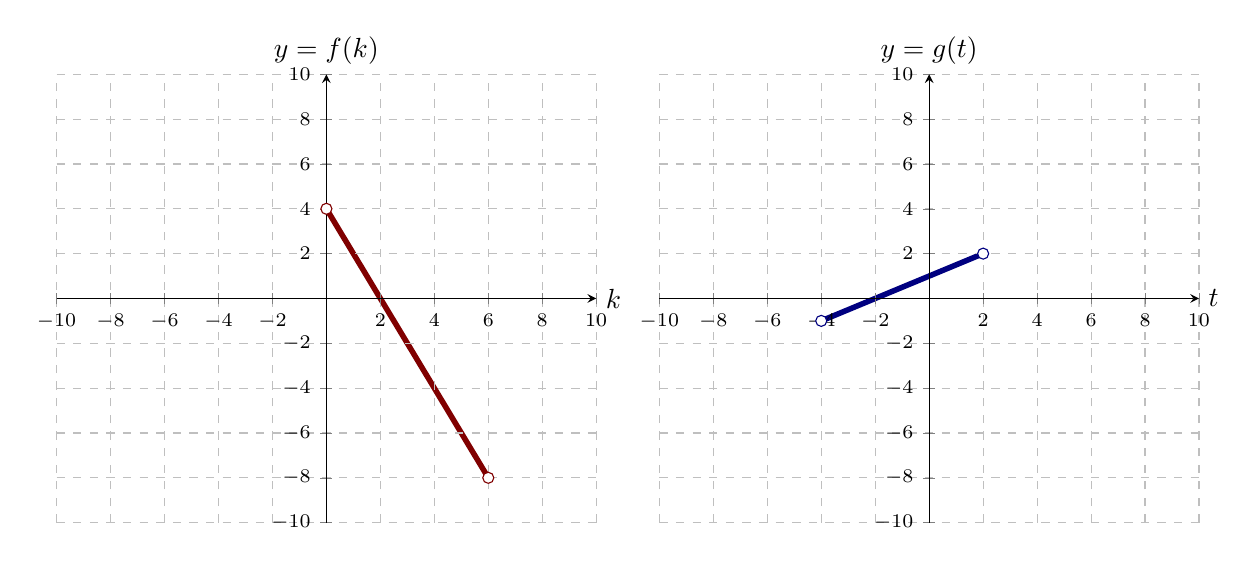
\begin{tikzpicture}
    \begin{axis}[name = sinax, domain=-10:10, ymax=10, xmax=10, ymin=-10, xmin=-10,
            axis lines =center, xlabel=$k$, ylabel={$y=f(k)$}, grid = major, grid style={dashed},
            ytick={-10,-8,-6,-4,-2,2,4,6,8,10},
            xtick={-10,-8,-6,-4,-2,2,4,6,8,10},
            yticklabels={$-10$,$-8$,$-6$,$-4$,$-2$,$2$,$4$,$6$,$8$,$10$}, 
            xticklabels={$-10$,$-8$,$-6$,$-4$,$-2$,$2$,$4$,$6$,$8$,$10$},
            ticklabel style={font=\scriptsize},
            every axis y label/.style={at=(current axis.above origin),anchor=south},
            every axis x label/.style={at=(current axis.right of origin),anchor=west},
            axis on top
          ]
          


          \addplot [line width=2, penColor2, smooth,samples=100,domain=(0:6)] ({x},{-2*x+4});
          \addplot [color=penColor2,fill=background, only marks,mark=*] coordinates{(0,4)};
          \addplot [color=penColor2,fill=background, only marks,mark=*] coordinates{(6,-8)}; 

           

    \end{axis}
    \begin{axis}[at={(sinax.outer east)},anchor=outer west, domain=-10:10, ymax=10, xmax=10, ymin=-10, xmin=-10,
            axis lines =center, xlabel=$t$, ylabel={$y=g(t)$}, grid = major, grid style={dashed},
            ytick={-10,-8,-6,-4,-2,2,4,6,8,10},
            xtick={-10,-8,-6,-4,-2,2,4,6,8,10},
            yticklabels={$-10$,$-8$,$-6$,$-4$,$-2$,$2$,$4$,$6$,$8$,$10$}, 
            xticklabels={$-10$,$-8$,$-6$,$-4$,$-2$,$2$,$4$,$6$,$8$,$10$},
            ticklabel style={font=\scriptsize},
            every axis y label/.style={at=(current axis.above origin),anchor=south},
            every axis x label/.style={at=(current axis.right of origin),anchor=west},
            axis on top
          ]
          
          \addplot [line width=2, penColor, smooth,samples=100,domain=(-4:2)] ({x},{0.5*x+1});
          \addplot [color=penColor,fill=background, only marks,mark=*] coordinates{(-4,-1)};
          \addplot [color=penColor,fill=background, only marks,mark=*] coordinates{(2,2)}; 


  \end{axis}

\end{tikzpicture}
\end{image}



To decide the function behavior of a composition, we need to follow movement through two graphs. \\



\[
(f \circ g)(x) = f(g(x))
\]



\textbf{\textcolor{blue!55!black}{Domain Movement in $g$:}}  First, we think of movement to the right in the domain of $f \circ g$.  This would be movement to the right in the domain of $g$.  The graph of $g$ is on the right above.  This would be movement to the right on the horizontal axis.



\textbf{\textcolor{blue!55!black}{Range Movement in $g$:}}  Next, according to the graph of $g$, as we move the right in the domain of $g$, the values of $g$ move up, which is to the right in the range of $g$.




\textbf{\textcolor{blue!55!black}{switch:}}   The range of $g$ becomes the domain of $f$.  


\textbf{\textcolor{blue!55!black}{Domain Movement in $f$:}}   The range of $g$ becomes the domain of $f$.  We were moving up on the graph of $g$, which means to the right in the range of $g$.  This switches to movement to the right in the domain of $f$.


\textbf{\textcolor{blue!55!black}{Range Movement in $f$:}}  Next, according to the graph of $f$, as we move the right in the domain of $f$, the values of $f$ move down, which is to the left in the range of $f$.  This is the range of $f \circ g$.




Gluing the whole story, movement to the right in the domain of $f \circ g$ corresponds to movement to the left in the range of $f \circ g$.

$f \circ g$ is a decreasing function.



\begin{observation}


This only applies to the domain of $f \circ g$, which needs to be determined. \\



The range of $g$ is $(-4, 2)$.  However, the domain of $f$ is $(0, 6)$.   We cannot use the whole range of $g$, which means we cannot use the whole domain of $g$.  Which part of the domain of $g$ does $g$ map into $(0, 6)$? \\


We need solutions to $g(t) = 0$.  From the graph, it looks like $g(-2) = 0$.  Therefore, we can only use $(-2, 2)$ from the domain of $g$.


Therefore, the domain of $f \circ g$ is $(-2, 2)$.  On this domain, $f \circ g$ is decreasing.



\end{observation}






\begin{warning}

Decreasing means the domain and range change in the opposite way.

When the domain increases, then range decreases.

It goes the other way as well.

When the domain decreases, the range increases.

They mean the same thing.


\end{warning}






We can describe all of this thinking algebraically as well. \\


If $a < b$ in the domain of $f \circ g$, then we want to know about $(f \circ g)(a)$  and $(f \circ g)(b)$.



\textbf{Step 1:}  If $a < b$, then $g(a) < g(b)$, because $g$ is an increasing function.


\textbf{Step 2:}  Now think of $g(a)$ and $g(b)$ as domain numbers for $f$.


\textbf{Step 3:}  If $g(a) < g(b)$, then $f(g(a)) > f(g(b))$, because $f$ is a decreasing function.


\textbf{Beginning to End:} If $a < b$, then $f(g(a)) > f(g(b))$ and $f \circ g$ is a decreasing function.














































\subsection*{Decreasing $\circ$ Decreasing}



$f$ and $g$ are defined graphically below.  $f$ and $g$ are both decreasing functions.  \\

What about $f \circ g$? \\



\begin{image}
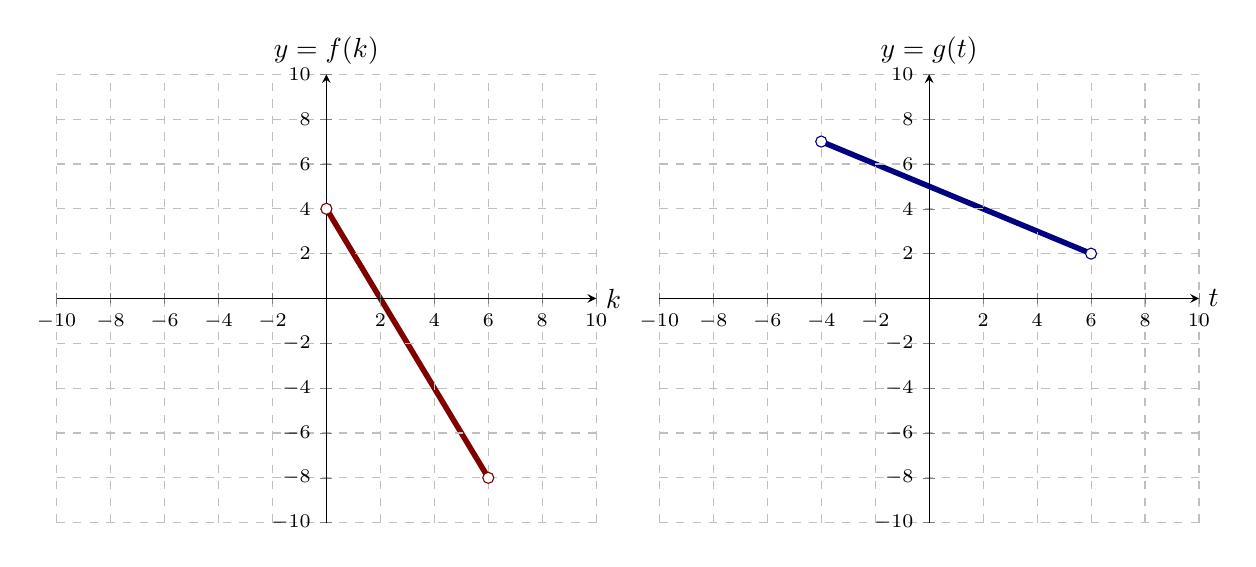
\begin{tikzpicture}
    \begin{axis}[name = sinax, domain=-10:10, ymax=10, xmax=10, ymin=-10, xmin=-10,
            axis lines =center, xlabel=$k$, ylabel={$y=f(k)$}, grid = major, grid style={dashed},
            ytick={-10,-8,-6,-4,-2,2,4,6,8,10},
            xtick={-10,-8,-6,-4,-2,2,4,6,8,10},
            yticklabels={$-10$,$-8$,$-6$,$-4$,$-2$,$2$,$4$,$6$,$8$,$10$}, 
            xticklabels={$-10$,$-8$,$-6$,$-4$,$-2$,$2$,$4$,$6$,$8$,$10$},
            ticklabel style={font=\scriptsize},
            every axis y label/.style={at=(current axis.above origin),anchor=south},
            every axis x label/.style={at=(current axis.right of origin),anchor=west},
            axis on top
          ]
          


          \addplot [line width=2, penColor2, smooth,samples=100,domain=(0:6)] ({x},{-2*x+4});
          \addplot [color=penColor2,fill=background, only marks,mark=*] coordinates{(0,4)};
          \addplot [color=penColor2,fill=background, only marks,mark=*] coordinates{(6,-8)}; 

           

    \end{axis}
    \begin{axis}[at={(sinax.outer east)},anchor=outer west, domain=-10:10, ymax=10, xmax=10, ymin=-10, xmin=-10,
            axis lines =center, xlabel=$t$, ylabel={$y=g(t)$}, grid = major, grid style={dashed},
            ytick={-10,-8,-6,-4,-2,2,4,6,8,10},
            xtick={-10,-8,-6,-4,-2,2,4,6,8,10},
            yticklabels={$-10$,$-8$,$-6$,$-4$,$-2$,$2$,$4$,$6$,$8$,$10$}, 
            xticklabels={$-10$,$-8$,$-6$,$-4$,$-2$,$2$,$4$,$6$,$8$,$10$},
            ticklabel style={font=\scriptsize},
            every axis y label/.style={at=(current axis.above origin),anchor=south},
            every axis x label/.style={at=(current axis.right of origin),anchor=west},
            axis on top
          ]
          
          \addplot [line width=2, penColor, smooth,samples=100,domain=(-4:6)] ({x},{-0.5*x+5});
          \addplot [color=penColor,fill=background, only marks,mark=*] coordinates{(-4,7)};
          \addplot [color=penColor,fill=background, only marks,mark=*] coordinates{(6,2)}; 


  \end{axis}

\end{tikzpicture}
\end{image}



To decide the function behavior of a composition, we need to follow movement through two graphs. \\



\[
(f \circ g)(x) = f(g(x))
\]



\textbf{\textcolor{blue!55!black}{Domain Movement in $g$:}}  First, we think of movement to the right in the domain of $f \circ g$.  This would be movement to the right in the domain of $g$.  The graph of $g$ is on the right above.  This would be movement to the right on the horizontal axis.



\textbf{\textcolor{blue!55!black}{Range Movement in $g$:}}  Next, according to the graph of $g$, as we move to the right in the domain of $g$, the values of $g$ move down, which is to the left in the range of $g$.




\textbf{\textcolor{blue!55!black}{switch:}}   The range of $g$ becomes the domain of $f$.  


\textbf{\textcolor{blue!55!black}{Domain Movement in $f$:}}   The range of $g$ becomes the domain of $f$.  We were moving down on the graph of $g$, which means to the left in the range of $g$.  This switches to movement to the left in the domain of $f$.


\textbf{\textcolor{blue!55!black}{Range Movement in $f$:}}  Next, according to the graph of $f$, as we move the left in the domain of $f$, the values of $f$ move up, which is to the right in the range of $f$.  This is the range of $f \circ g$.




Gluing the whole story, movement to the right in the domain of $f \circ g$ corresponds to movement to the right in the range of $f \circ g$.

$f \circ g$ is a increasing function. \\


Decreasing means turning around and we turned around twice. \\


\begin{observation}


This only applies to the domain of $f \circ g$, which needs to be determined. \\



The range of $g$ is $(2, 7)$.  However, the domain of $f$ is $(0, 6)$.   We cannot use the whole range of $g$, which means we cannot use the whole domain of $g$.  Which part of the domain of $g$ does $g$ map into $(0, 6)$? \\


We need sa olution to $g(t) = 6$.  From the graph, it looks like $g(-2) = 6$.  Therefore, we can only use $(-2, 6)$ from the domain of $g$.


Therefore, the domain of $f \circ g$ is $(-2, 6)$.  On this domain, $f \circ g$ is decreasing.



\end{observation}






\begin{warning}

Decreasing means the domain and range change in the opposite way.

When the domain increases, then range decreases.

It goes the other way as well.

When the domain decreases, the range increases.

They mean the same thing.


\end{warning}






We can describe all of this thinking algebraically as well. \\


If $a < b$ in the domain of $f \circ g$, then we want to know about $(f \circ g)(a)$  and $(f \circ g)(b)$.



\textbf{Step 1:}  If $a < b$, then $g(a) > g(b)$, because $g$ is a decreasing function.


\textbf{Step 2:}  Now think of $g(a)$ and $g(b)$ as domain numbers for $f$.


\textbf{Step 3:}  If $g(a) > g(b)$, then $f(g(a)) < f(g(b))$, because $f$ is a decreasing function.


\textbf{Beginning to End:} If $a < b$, then $f(g(a)) < f(g(b))$ and $f \circ g$ is an increasing function.







































\begin{center}
\textbf{\textcolor{green!50!black}{ooooo-=-=-=-ooOoo-=-=-=-ooooo}} \\

more examples can be found by following this link\\ \link[More Examples of Composition]{https://ximera.osu.edu/csccmathematics/precalculus2/precalculus2/composition/examples/exampleList}

\end{center}






\end{document}
